\chapter{Technische Charakteristiken und Spezifikationen}

\section{Allgemeines Design und technische Voraussetzungen}

\subsection{Technische Limitationen High Frequency RFID}
Für HF Tags (wie diejenigen die auch in der Speicherbibliothek verwendet werden) ist die Betriebsfrequenz durch den ISO Standard 18000-3 auf 13.56MHz festgelegt und typische Lesereichweiten liegen bei etwa einem Meter \parencite{chawla2007}.

Um weitere technische Limitation zu erkennen wurden, mit der Hardware von Hyientech, verschiedene Versuche (siehe Anhang \ref{app:ch:Versuche}) durchgeführt, welche zu folgenden Erkenntnisse geführt haben:

\begin{itemize}
	\item Distanz zwischen gestapelten Tags muss mindestens 3cm betragen.
	\item Distanz zwischen aneinandergereihten Tags muss mindestens 1cm betragen.
	\item Winkel zwischen Tag und Antenne darf nicht grösser als 60\SIUnitSymbolDegree sein.
	\item Tags, welche sich hinter Metall befinden, können nicht erkennt werden.
	\item Maximale Distanz nur bei optimalen Winkel zwischen Antenne und Tag möglich.
\end{itemize}

\subsection{Hardware}
Die Hardware besteht aus einem RFID Lesegeräte, mit zwei angeschlossenen Antennen. Eine der beiden Antennen soll sich, auf Höhe der Wiegestation, direkt neben dem Förderband befinden. Die Zweite Antenne soll sich am Ende des Förderbandes befinden, sodass ein Winkel von 90\SIUnitSymbolDegree erreicht wird, um die Tags, welche sich in der Flucht des Förderbands befinden, lesen zu können (siehe Abbildung \ref{fig:positionAntennen}). Um zu verhindern, dass Behälter, welche sich auf dem benachbarten Förderband befinden, ausgelesen werden, wird zwischen den beiden Förderbändern eine einfache Aluminiumplatte platziert (siehe Abbildung \ref{fig:positionAntennen}). Die durchgeführten Versuche haben ergeben, dass diese ausreicht, um ein Auslesen der Tags dahinter zu verhindern.

\begin{figure}[htb]
	\centering
	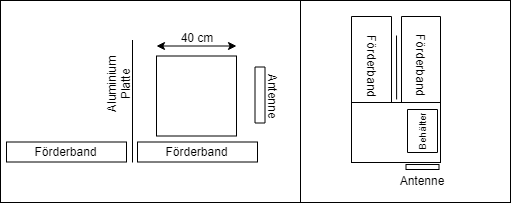
\includegraphics[keepaspectratio,width=\linewidth]{Positionierung_Antennen}
	\caption{Antennenposition Eins und Zwei}
	\label{fig:positionAntennen}
\end{figure}

Die Platzierung der Antennen steht in direktem Einfluss mit der Lesbarkeit der Tags, da die Ausrichtung der Tags im Verhältnis zur Antenne dazu führen kann, dass dieser nicht gelesen werden kann. Deshalb kann durch den Einsatz mehrerer Antennen gewährleistet werden, dass die Tags der am häufigsten im Hochregallager vorzufindenden Lagermöglichkeiten gelesen werden können (siehe Abbildung \ref{fig:lagermöglichkeitExemplare}).

\begin{figure}[htb]
	\centering
	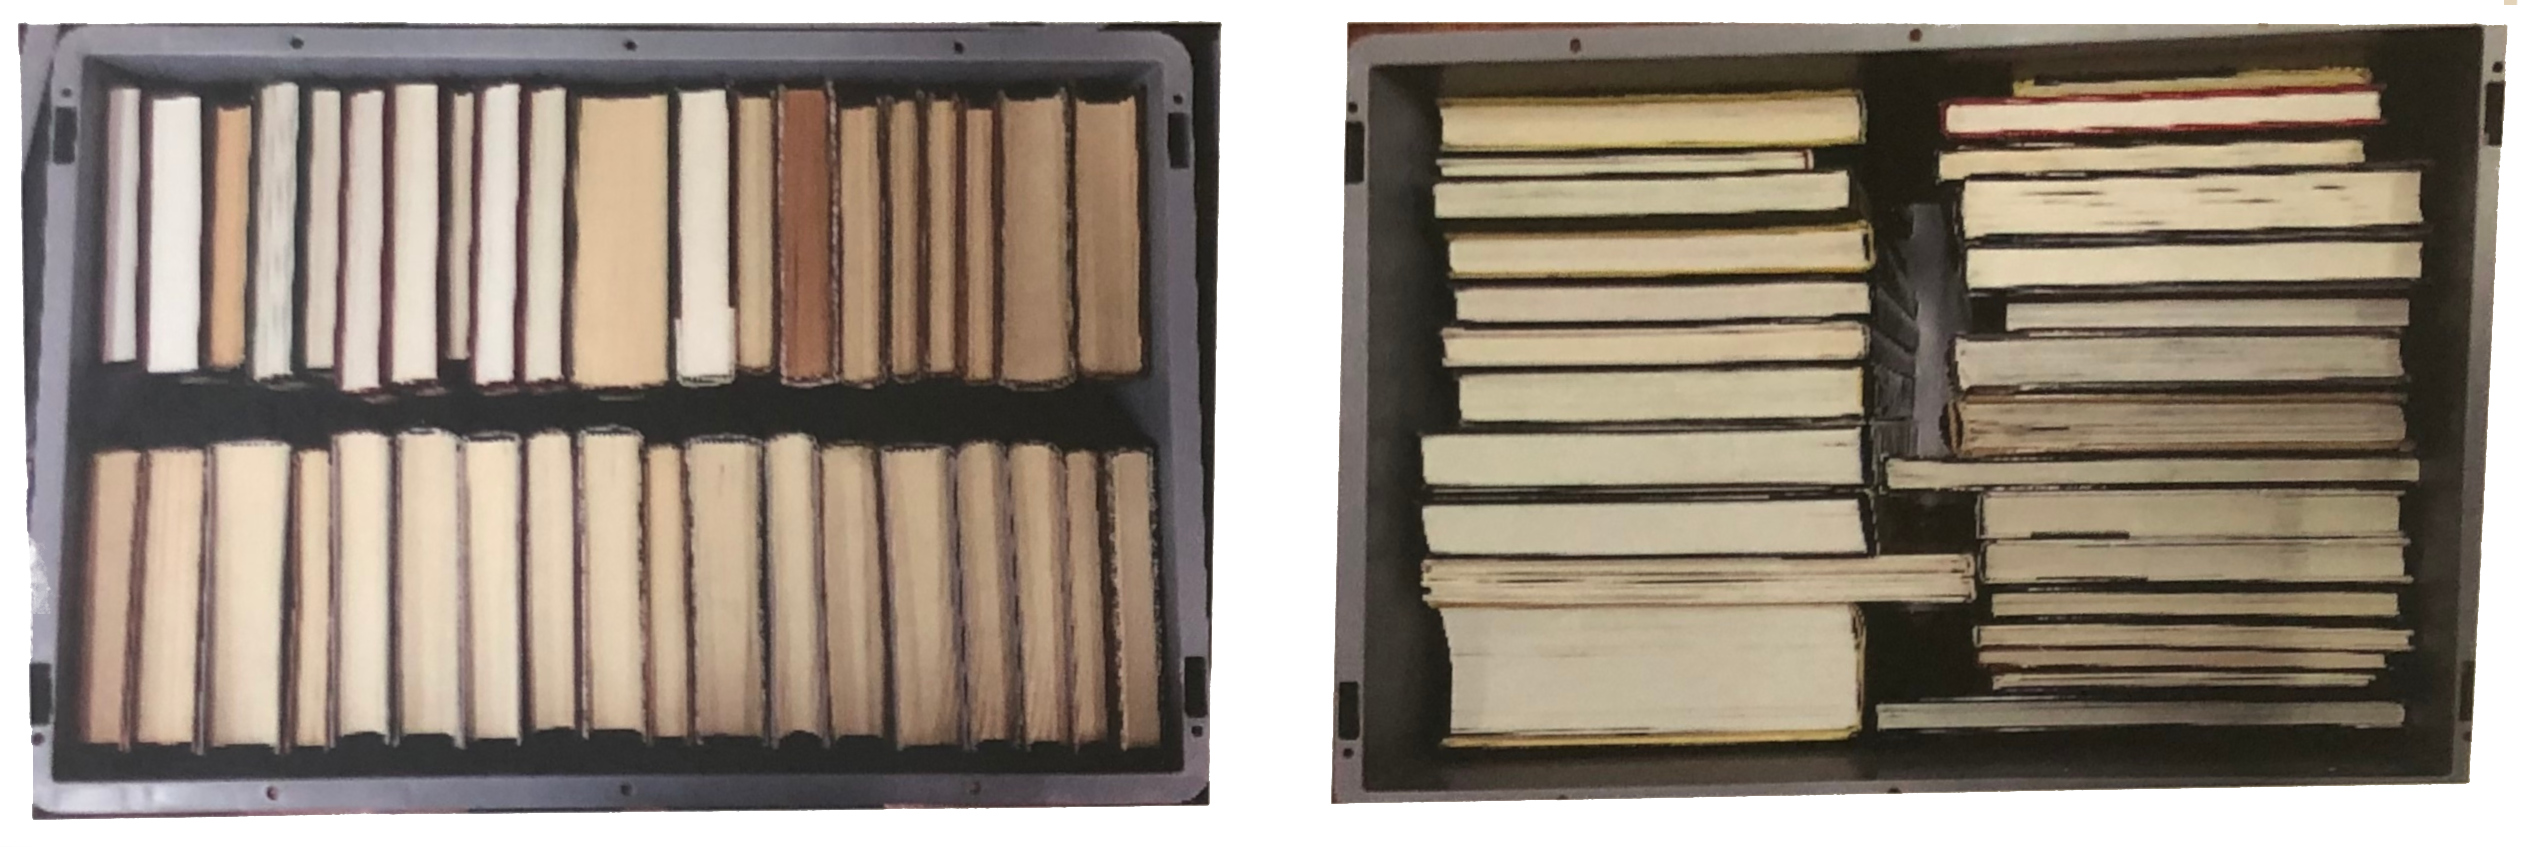
\includegraphics[keepaspectratio,width=\linewidth]{Lagerung_Exemplare}
	\caption{Meistgenutzte Lagermöglichkeiten von Exemplaren}
	\label{fig:lagermöglichkeitExemplare}
\end{figure}

Durch die Ausrichtung der Antennen wird weiter vorausgesetzt, dass das Lesegerät mit den Antennen eine maximale Distanz von circa 65cm lesen können. Jeder Behälter enthält gemäss Angaben im Schnitt 50 Exemplare. Daraus ergibt sich, dass das Lesegerät 50 Exemplare in der Zeit auslesen muss, welche das Förderband benötigt um den Behälter circa 60cm weit zu transportieren.

\section{Vergleich der vorgeschlagenen Lösung und der existierenden Situation}
Die existierende Situation enthält momentan noch keine Möglichkeit der Verifikation des Inhaltes eines Behälters. Demnach würde durch die Durchführung dieses Projektes die Wahrscheinlichkeit des Deplatzieren eines Exemplares, in einen nicht vorgesehenen Behälter, verringern.

\section{Vorteile und deren Gründe der vorgeschlagenen Lösung}
\begin{itemize}
	\item Durch die Rückbeziehung, welche über die Mehrheit der gelesenen Tags Rückschlüsse auf die ID der Behälter zulässt, kann auf einen Barcodeleser verzichtet werden. Dies ermöglicht eine positionsunabhängige Erkennung des Behälters.
	\item Die direkte Aussortierung des Behälters bringt mehrere Vorteile. So wird der bereits bestehende Prozess des Aussortierens, mit welchem die Mitarbeiter vertraut sind, verwendet. Das Aussortieren geschieht zurzeit bei Behältern, welche Exemplare enthalten die über den Behälterrand hinwegschauen, sowie bei Behältern, welche zu schwer sind. Weiter führt der Umstand der direkten Aussortierung dazu, dass keine weiteren Fehlerquellen durch zusätzliche manuelle Interaktion durch einen Mitarbeiter entstehen. Ein weiterer Vorteil liegt darin, dass die Erkennung sehr früh geschieht, da die Aussortierung noch vor der Einlagerung des Behälters stattfindet.
	\item Der Einsatz mehrerer Antennen bringt den Vorteil, dass Tags mit verschiedenen Ausrichtungen identifiziert werden können. Dies aus dem Grund, dass sich die Tags bei unterschiedlichen Ausrichtungen unterschiedlich stark beeinflussen. Weiter kann durch den Einsatz mehrere Antennen der Suchradius vergrössert werden. Dies führt zu dem Umstand, dass sich der Behälter länger in einem Suchradius befindet, wodurch mehr Zeit für die Inventarisierung der Tags zur Verfügung steht. Deshalb können insgesamt mehr Tags identifiziert  werden.
	\item Die Installation der RFID Antennen soll, wie in Abbildung \ref{fig:positionAntennen} ersichtlich, für die erste Antenne gleich bei der Eckpartie und für die zweite unmittelbar nach der Wiegestation erfolgen. Dies bringt den Vorteil, dass mehr Zeit für die Inventarisierung zur Verfügung steht, da der Behälter für eine kurze Zeit auf der Waage still steht. Weiter ist mit keiner Interferenz durch andere Behälter oder Objekte, wie Metall, zu rechnen, da sich nur Luft zwischen der Antenne und dem Behälter befindet. Zudem können durch die Unterschiedlichen Ausrichtungen der Antennen mehr Tags Identifiziert werden.
\end{itemize}


\section{Vorgeschlagene Zulieferungsquellen}
\label{sec:VorschlagQuellen}
Als Zulieferungsquelle für die RFID Hardware wird zu Feig Electronis geraten, da dieser Hersteller im Vergleich mit weiteren in Europa ansässigen Unternehmen ein gutes Preisleistungsverhältnis aufzeigt. Durch die Ortsnähe kann bei Garantiefällen ein speditiver vor Ort Support gewährleistet werden. Weiter spricht auch der Umstand, dass RFID Lösungsanbieter wie Bibliotheka auf Feig Electronis als Hersteller vertrauen, für diesen Lieferanten.

Für die Anpassung des Lagerverwaltungssystems muss aufgrund der bestehenden Infrastruktur auf Stöcklin zurückgegriffen werden.

Die Umsetzung des Projektes der Implementierung des untersuchten Konzeptes soll durch eine weitere Bachelorarbeit an einer Hochschule umgesetzt werden. Dies bedingt durch das vorhandene Lernpotential sowie die tiefen Kosten einer studentischen Arbeit an einer Hochschule.

\section{Geschätzte Kosten und Quellen für die Basis dieser Schätzungen}
\subsection{Hardware}
\label{ssec:HardwareKosten}
\begin{tabularx}{\textwidth}{|r|X|r|r|}
	\hline
	\textbf{Menge} & \textbf{Produkt} & \textbf{Kosten(CHF)} & \textbf{Kosten gesamt(CHF)} \\
	\hline
	1 & RFID Reader ID ISC.LR2500-A (Feig) & 1'300 & 1'300 \\
	\hline
	2 & RFID Antennen ID ISC.ANT800/600 (Feig)& 830 & 1'660 \\
	\hline
	2 & RFID Antennenkabel ID ISC.ANT.C-A (Feig) & 22 & 44 \\
	\hline
	1 & RFID Multiplexer 8-fach HF Multiplexer (Feig) & 540 & 540 \\
	\hline
	1 & Netzteil ID NET.24V-B (Feig) & 33 & 33 \\
	\hline
	1 & Netzkabel ID CAB.NET.24V-B-EU (Feig) & 5 & 5 \\
	\hline
	& & & \textbf{3'582} \\
	\hline
\end{tabularx}

Die Kosten dieser Schätzung aller Feig Electronics Artikel basieren auf der eingeholten Offerte (Siehe Abbildung \ref{fig:offerteFeig}), bei welcher EUR in CHF mit einem Wechselkurs von 1.14 auf welchem noch 7.7\% MwSt. hinzugerechnet wurden.
Für die weiteren Artikel wurde auf den in der Tabelle ersichtliche Webseiten, die Kosten für das jeweilige Produkt herausgeschrieben (Besuch der Webseiten am 08.05.2019).

\begin{figure}[htb]
	\centering
	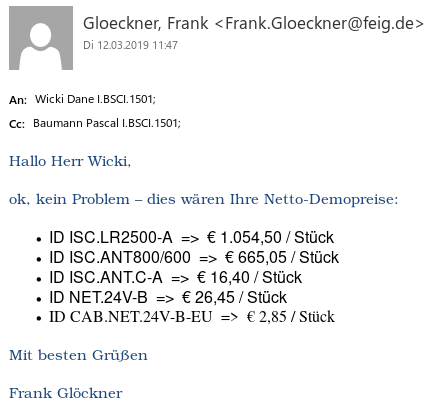
\includegraphics[keepaspectratio,width=.5\linewidth]{Screenshot_Email_Feig}
	\caption{E-Mail der Offerte}
	\label{fig:offerteFeig}
\end{figure}

\subsection{Software}
\label{ssec:SoftwareKosten}
\begin{tabularx}{\textwidth}{|r|r|X|r|}
	\hline
	\textbf{Stunden(h)} & \textbf{Lohn(CHF/h)} & \textbf{Beschrieb} & \textbf{Kosten gesamt(CHF)} \\
	\hline
	50 & 200 & Umsetzung, sofern die Software die Befehle bereits über das Netzwerk entgegennimmt. & 10'000 \\
	\hline
	250 & - & Umsetzung des Projektes von einem Studenten im Rahmen einer Bachelorarbeit & 1'000 \\
	& & & \textbf{11'000} \\
	\hline
\end{tabularx}

Die verwendeten Stundenkosten basieren auf aufgerundeten Werten, welche ein Freelancer in der Schweiz verdienen kann.
Für die Kosten der Bachelorarbeit wurden die Kosten übernommen, welche die Hochschule Luzern für deren Durchführung für eine Bachelorarbeit mit einem einzelnen Studenten verrechnet.
